\section{Catalogue des solutions et tests effectués}
\subsection{Pré-étude des micro-capsules}

Les micro-capsules sont fabriqué à partir de verre borosilicate 3.3 (voir Annexe \ref{pdf:borosilicate}), ce type 
de verre est souvent utilisé pour la verrerie de laboratoire. En effet, il comporte une 
très bonne résistance aux chocs thermique du faite de son faible coefficient de dilatation. 
De plus, il est résistant à de nombreux produits chimiques.
Néanmoins, son comportement mécanique peut s'avéré fragile en particulier pour de faibles
épaisseurs (voir \cite{report_borosilicate}).

\vspace{0.3cm}

\begin{figure}[H]
    \centering
    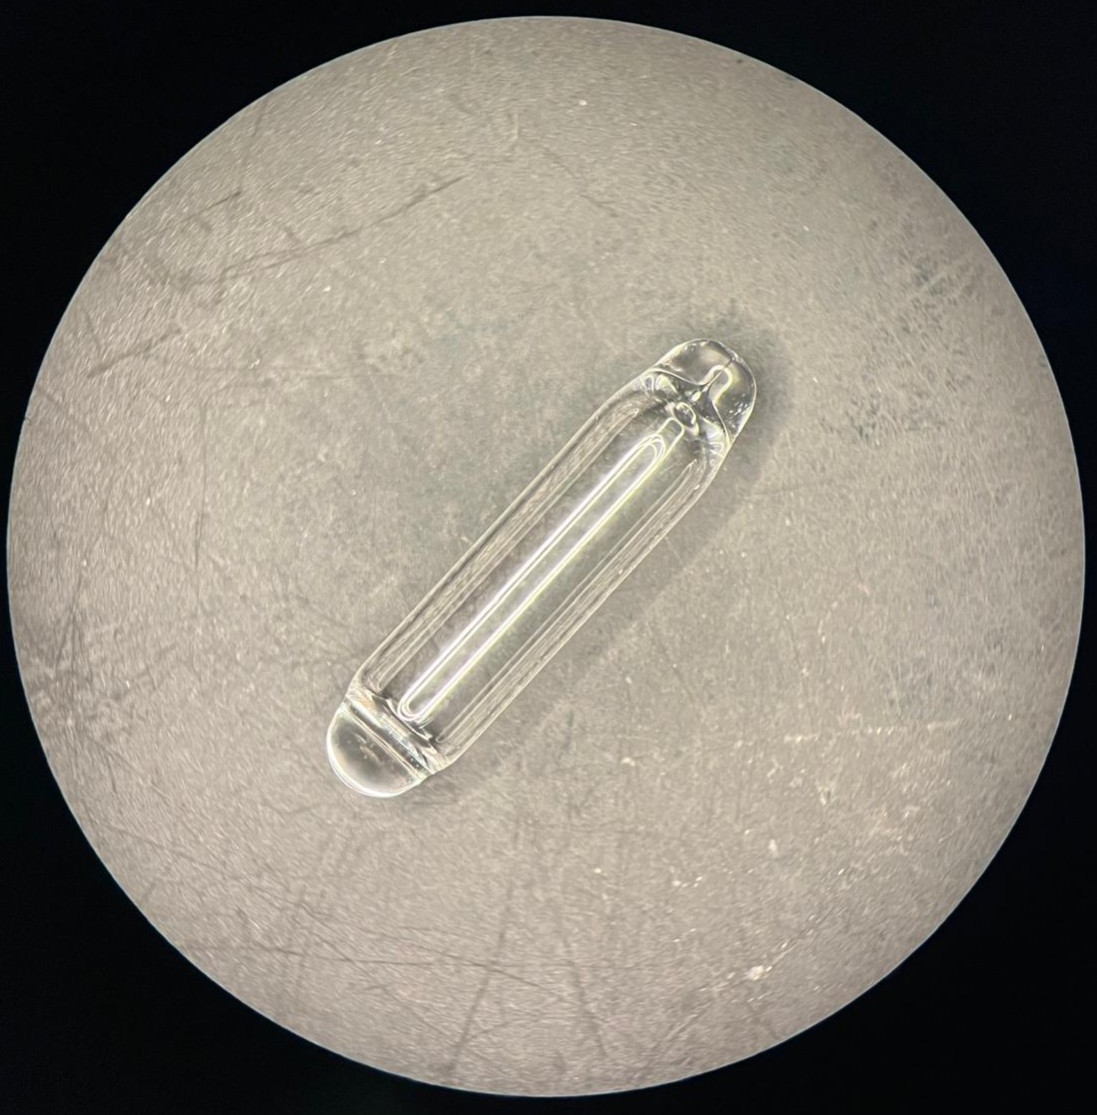
\includegraphics[width=7cm]{Images/Illustrations/CDH/Micro-capsule.jpg}
    \label{fig:microcapsule_loupe}
    \caption{Observation d'une micro-capsule avec une loupe binoculaire}
\end{figure}

Les micro-capsules seront fermée à terme par une entreprise externe à l'aide d'une machine laser permettant de sceller le verre.
Cependant pour le moment, par soucis de simplicité, les micro-capsules sont fermée manuellement grâce à une 
perceuse à colonne et un chalumeau.

\begin{figure}
    \centering
    \begin{subfigure}[b]{0.4\textwidth}
        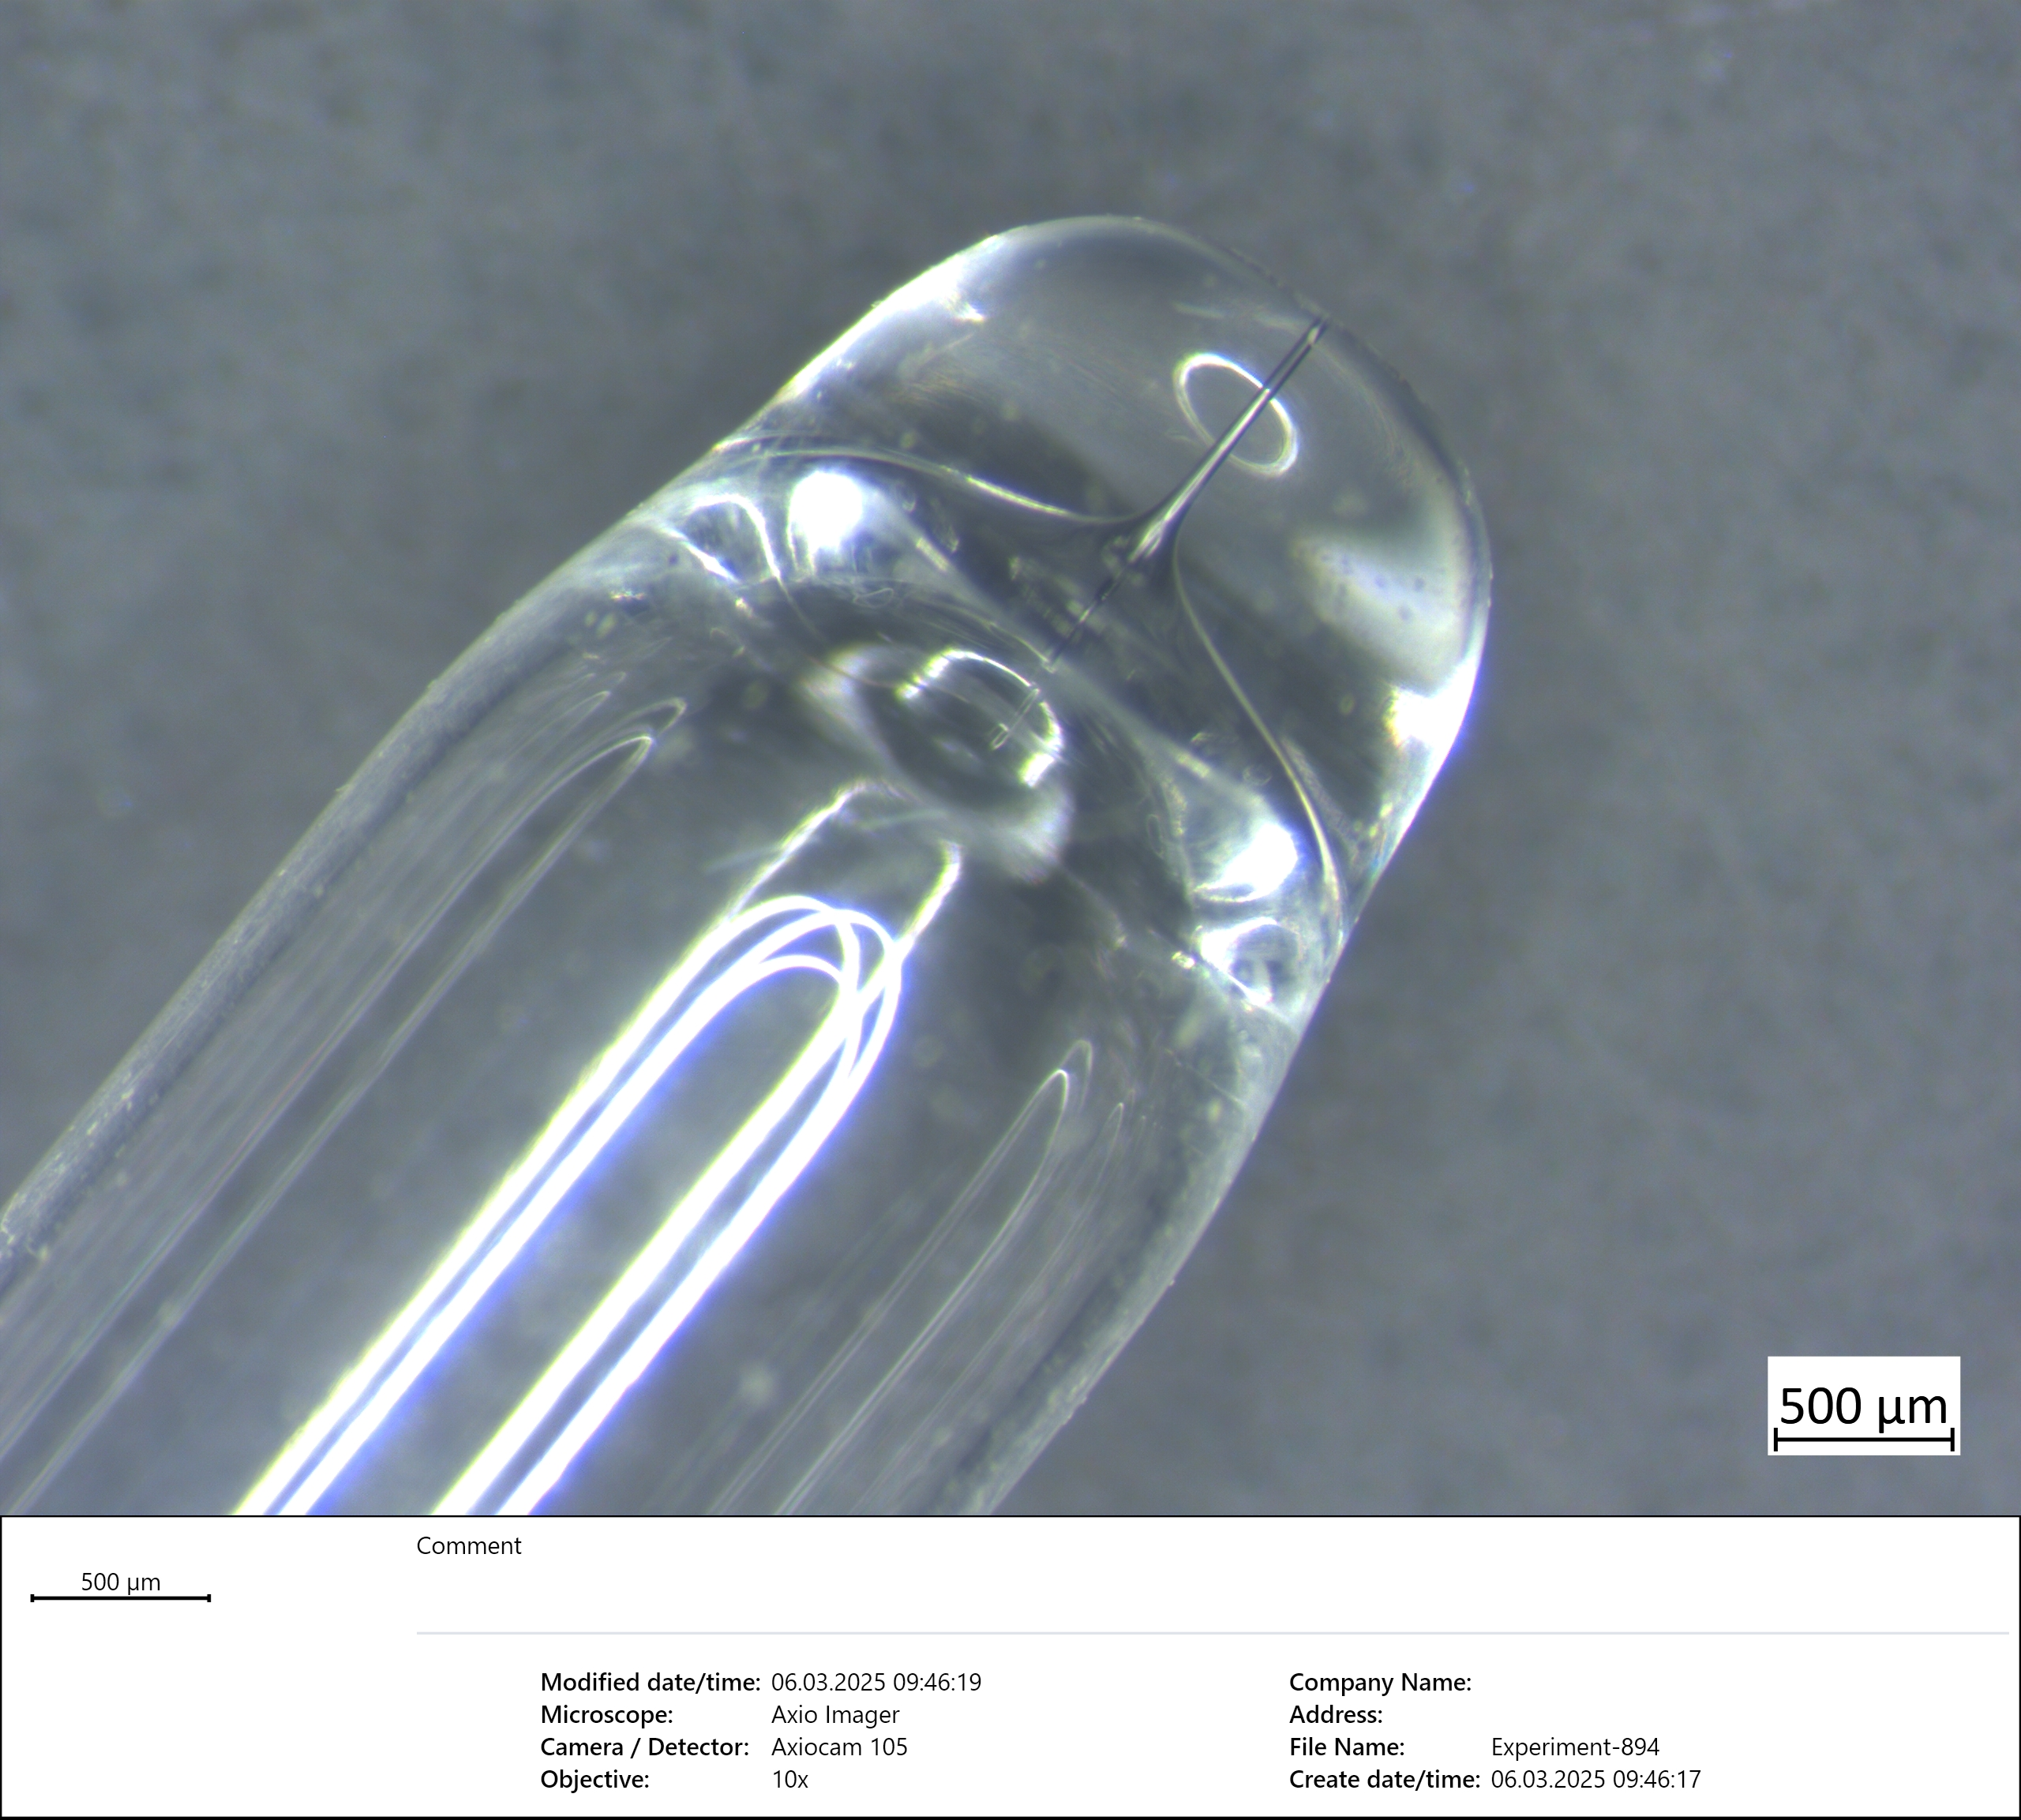
\includegraphics[width=6cm]{Images/Illustrations/CDH/MicroCapsule_trou.jpg}
        \caption{Micro-capsule mal fermée observé au microscope}
        \label{fig:trou_microcapsule}
    \end{subfigure}
    \begin{subfigure}[b]{0.4\textwidth}
        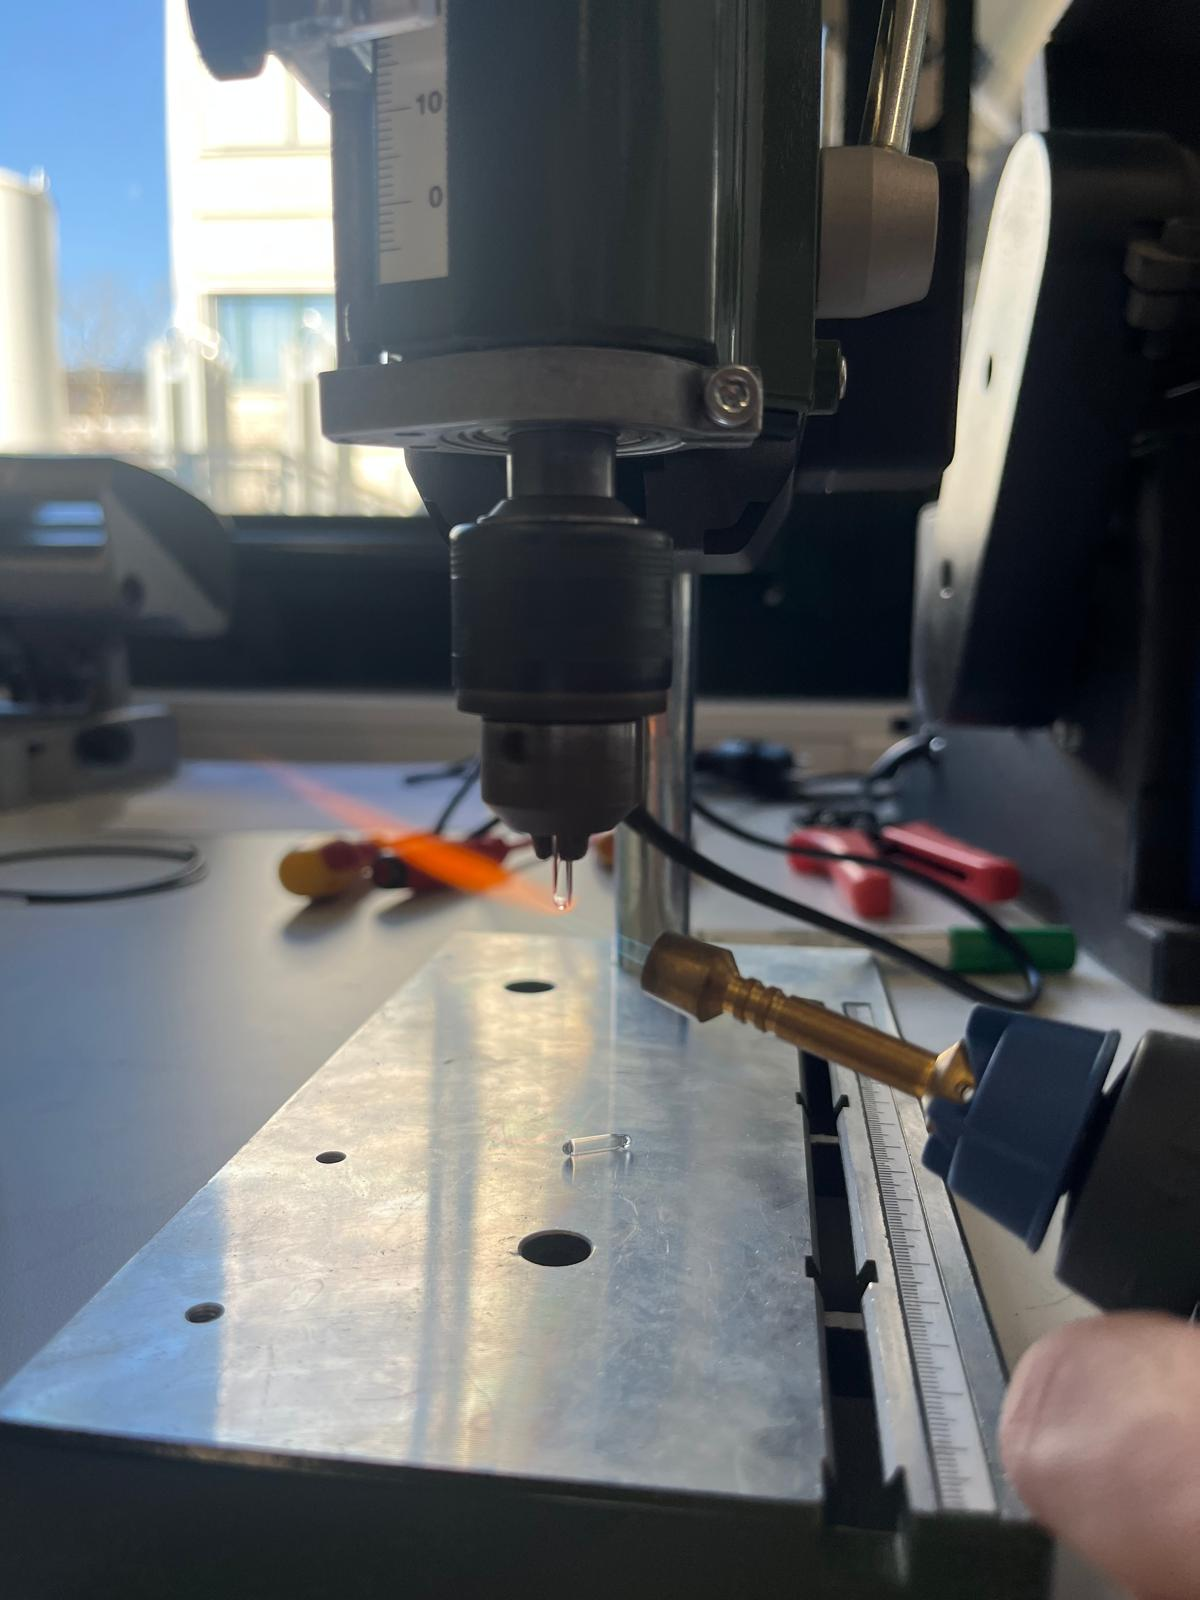
\includegraphics[width=6cm]{Images/Illustrations/CDH/Fermeture_capsule.jpg}
        \caption{Fermeture d'une micro-capsule avec le chalumeau}
        \label{fig:chalumeau}
    \end{subfigure}
    \caption{Fermeture manuel des micro-capsules}
    \label{fig:fermeture_microcapsule}
\end{figure}




\subsection{Liste des solutions envisagées}
\subsubsection{Canon à azote}
\paragraph{Principe de la solution}
L'idée de cette solution est de placer la micro-capsule dans un tube, puis de la soumettre à une pression d'azote élevée.
Ce qui aura pour effet de propulser la micro-capsule contre le fond du réacteur.

\paragraph{Tests et simulations}
Prototype réalisé en impression 3D (voir figure \ref{fig:proto_canon}).
Des tests ont été effectués avec une pression de 4 bar dans le tube.

\begin{figure}[H]
    \centering
    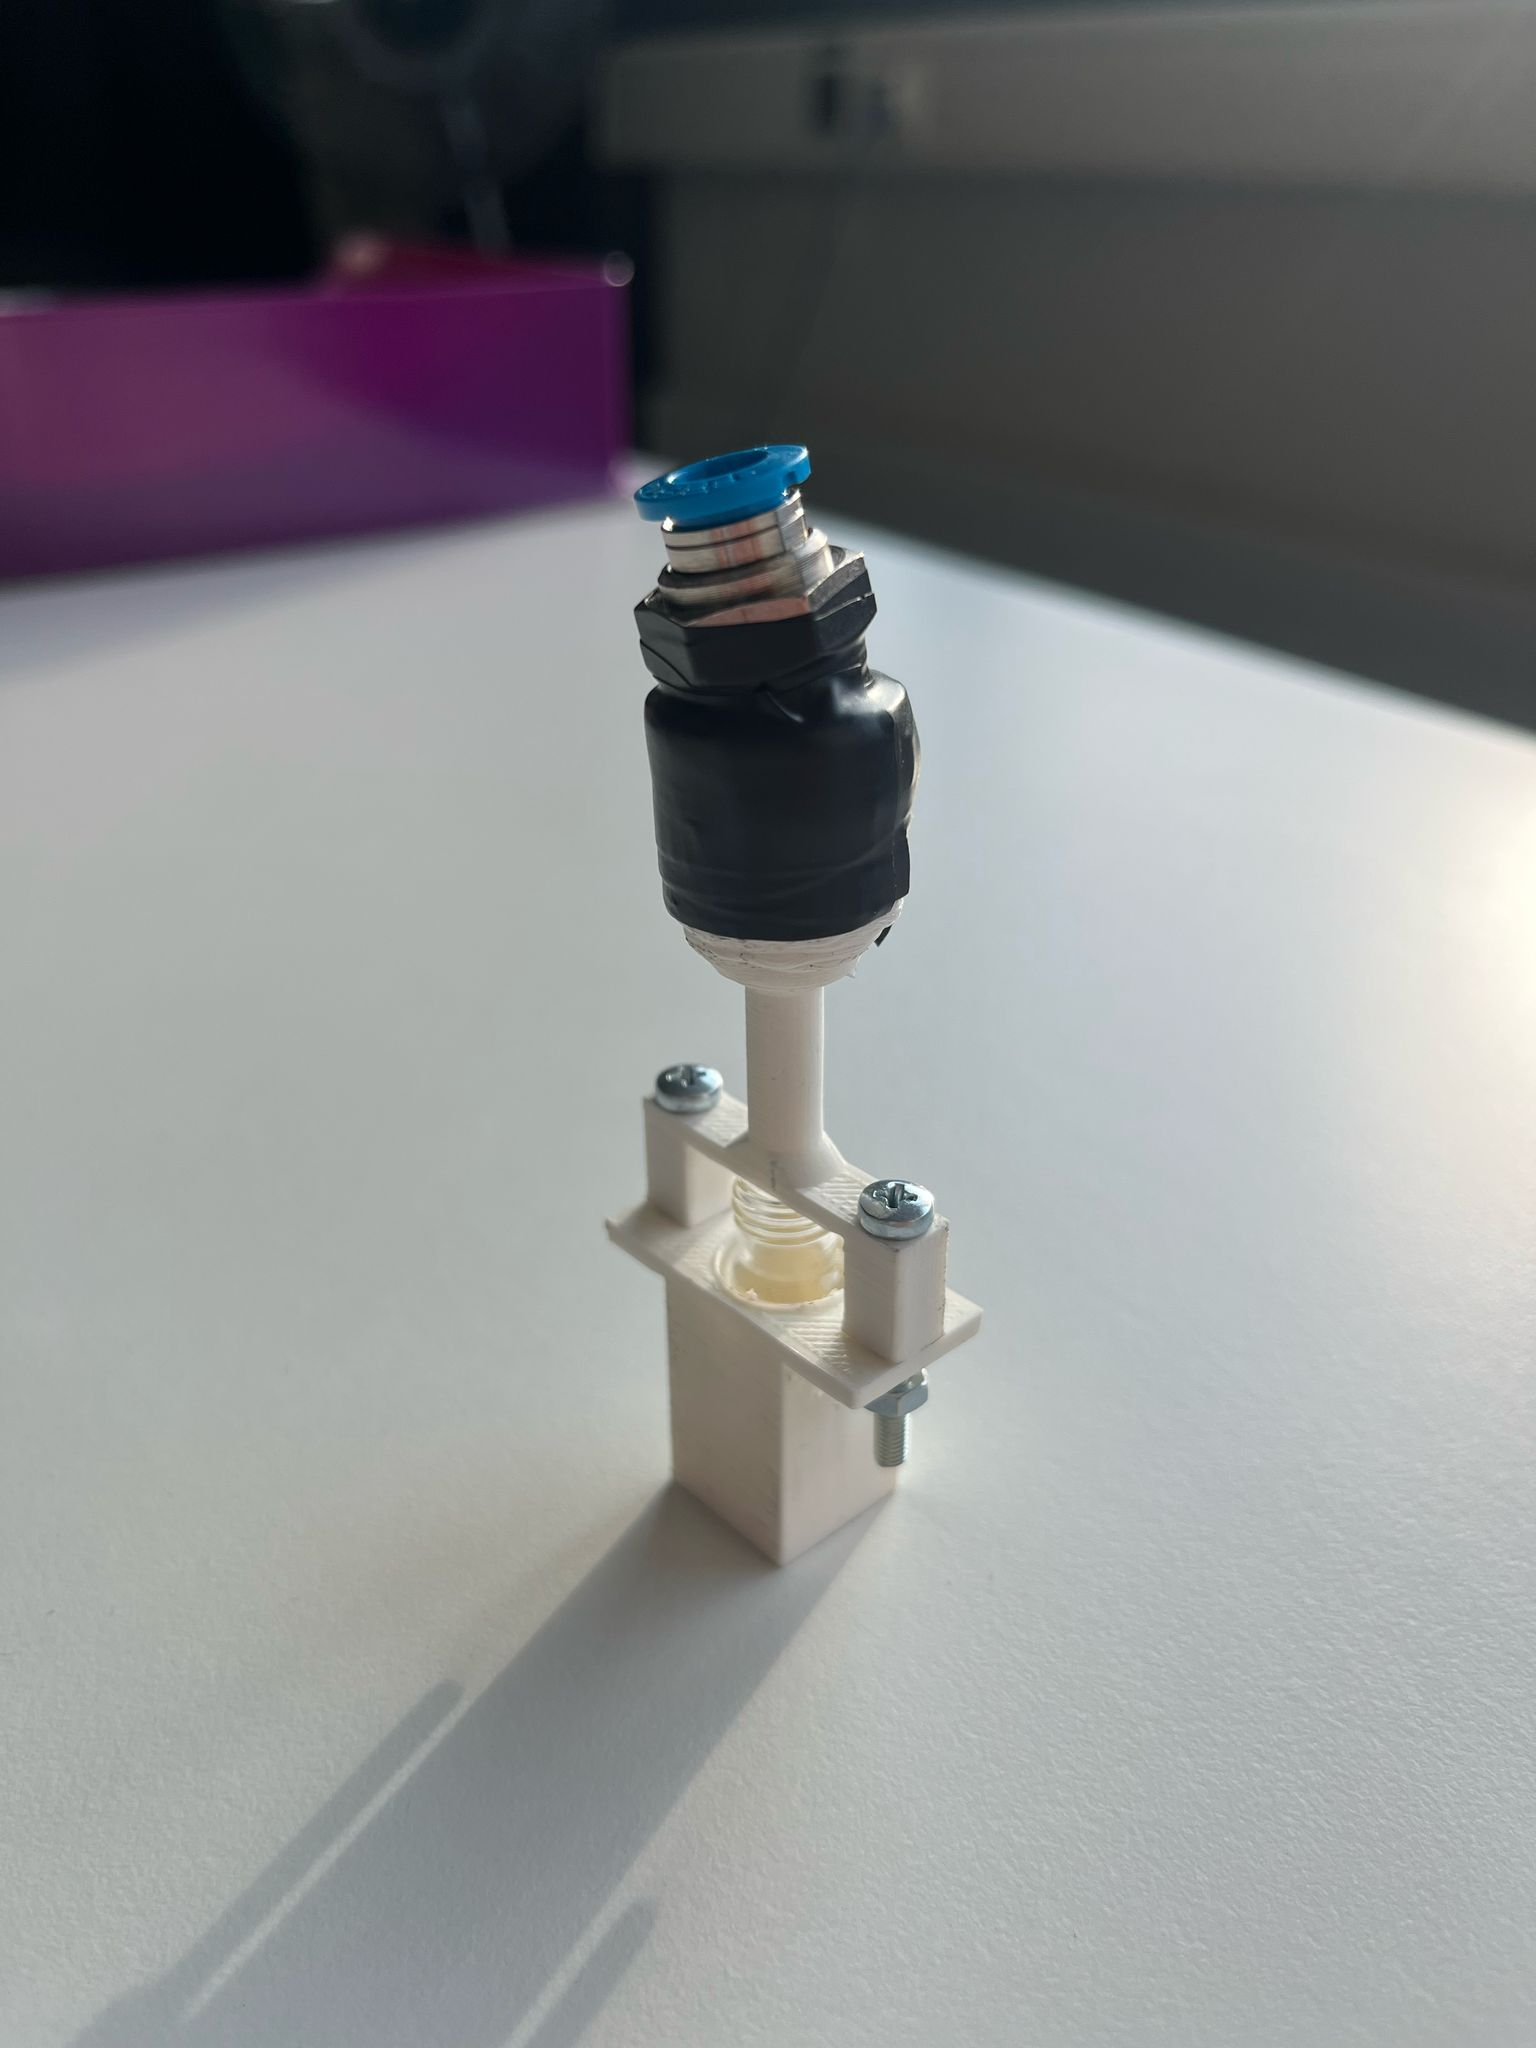
\includegraphics[width=6cm]{Images/Illustrations/Solutions/Proto_canon.jpg}
    \caption{Prototype du canon à azote}
    \label{fig:proto_canon}
\end{figure}

Puis d'autres tests ont été réalisé avec de l'azote à une pression de 7 bar.
A cette pression la micro-capsule c'est parfaitement brisée. Cependant, le fond du réacteur à également été brisée. 
(voir figure \ref{fig:fond_reacteur})

\begin{figure}[H]
    \centering
    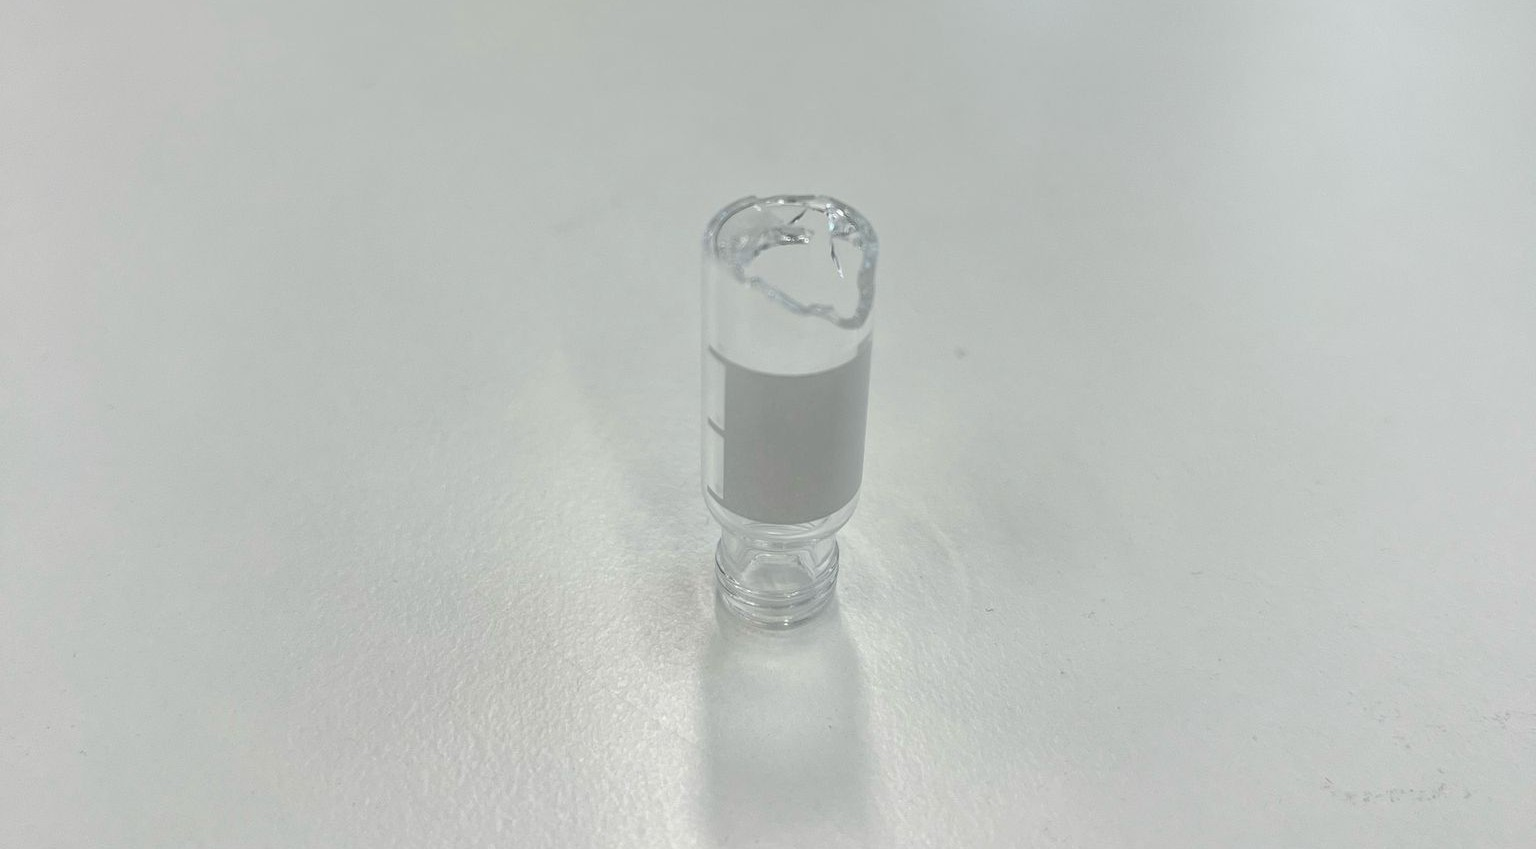
\includegraphics[width=9cm]{Images/Illustrations/Solutions/Reacteur_casse.jpg}
    \caption{Fond du réacteur brisé après test à 7 bar}
    \label{fig:fond_reacteur}
\end{figure}


\paragraph{Conclusion}
En conclusion, lors des essais réalisé, la micro-capsule ne s'est pas brisée pour des pressions inférieures à 4 bar.


En outre, après discutions au-près des chimistes, le risque de cross-contamination est trop élevé, dû aux éclats de verre et à certains réactifs très volatiles.
Enfin, la complexité de la mise en place de cette solution pour une application de pick and place est trop importante. 
Ce qui rend cette solution non viable pour le projet.

\subsubsection{Implosion de la capsule}
\paragraph{Principe de la solution}
Le principe de cette solution est de placer tout les réacteurs contenant des micro-capsules dans une chambre que
l'on va soumettre à une forte pression. Cette pression devrait provoquer l'implosion des micro-capsules.

\paragraph{Tests et simulations}
Une chambre de mise sous pression utilisé pour de précédents tests à été réutilisé.


\begin{table}[H]
    \centering
    \begin{tabular}{|l|l|}
    \hline
    \rowcolor[HTML]{C1EB5F} 
    \multicolumn{1}{|c|}{\cellcolor[HTML]{C1EB5F}\textbf{Avantages}} &
      \multicolumn{1}{c|}{\cellcolor[HTML]{E4AAAB}\textbf{Inconvenients}} \\ \hline
    \begin{tabular}[c]{@{}l@{}}Cassage des capsules effectué \\ directement dans le réacteur.\end{tabular} &
      \begin{tabular}[c]{@{}l@{}}Nécessite une pression assez\\ élevée.\end{tabular} \\ \hline
    \begin{tabular}[c]{@{}l@{}}Peu ou pas de cross-contamination \\ si implosion contrôlée.\end{tabular} &
      \begin{tabular}[c]{@{}l@{}}Simulation et comportement\\ plus complexe.\end{tabular} \\ \hline
    \end{tabular}
    \caption{Avantages et inconvénients du cassage par pression}
    \label{tab:AvIncPression}
    \end{table}

\paragraph{Conclusion}


\newpage
\subsubsection{Actionneur mécanique}
\paragraph{Principe de la solution}
Pour cette solution, l'idée est d'ouvrir simplement les micro-capsules à l'aide de 48 mini pistons, 
sur lesquels des petits disques en verre (consommable), sont maintenu par un système d'aspiration.

\vspace{0.3cm}
Le but de ces disques est d'évité la cross contamination entre les différents réacteurs et de limiter le retour 
des projections.

\vspace{0.3cm}
Le cycle de fonctionnement typique de cette solution serai le suivant :
\begin{enumerate}
    \item Un distributeur vient placer un disque sur chaque piston.
    \item Les pistons active l'aspiration et les disques sont maintenus.
    \item Les pistons descendent et viennent percuter les micro-capsules.
    \item Les disques sont relâchés et les pistons remontent.
    \item Les pistons retournent à leur position initiale.
\end{enumerate}

\paragraph{Tests et simulations}

\paragraph{Conclusion}

\subsubsection{Fréquence de résonance}
\paragraph{Principe de la solution}
Le principe de cette solution est de placer un haut parleur à proximité des micro-capsules puis de les faire vibrer à leurs fréquence de résonance.
Ce qui devrait avoir pour effet de les briser.


\paragraph{Tests et simulations}
Après avoir discuté avec M. Costanzo, la solution pourrait s'avéré complexe car toutes les micro-capsules ne sont
pas exactement identique du faite de la fermeture. Elle risque de ne pas toute vibrer à la même fréquence de résonance.

\vspace{0.3cm}
Par ailleurs, leur forme cylindrique fermée à chaque extrémité rigidifie grandement la structure et rend difficile l'entrée
en résonance.

\paragraph{Conclusion}
Aucun test pratique n'a été réalisé pour cette solution.


\subsection{Critères et choix de la solution}
